\documentclass[11pt, a4paper, twoside, openany]{tfg_dtic_upf}

%FONT ENCODING (T1: proper accented glyphs, correct copy-paste and hyphenation of accented words)
\usepackage[T1]{fontenc}

%LANGUAGES (last listed is the main language: English)
\usepackage[spanish,catalan,english]{babel}

% Page layout: ~2.5 cm margins
\usepackage{geometry}
\geometry{
  a4paper,
  top=2.5cm,
  bottom=2.5cm,
  inner=2.5cm,
  outer=2.5cm
}

% Avoid inserted blank verso pages in twoside mode
\let\cleardoublepage\clearpage

% No first-line indent on new paragraphs
\setlength{\parindent}{0pt}

%GRAPHICS AND LOGO
\usepackage{graphicx}
\graphicspath{{figures/}{template/}}

%FONT: TIMES
\usepackage{times}

%MATHEMATICS
\usepackage{amsmath,amssymb,amsthm}

%TABLES
\usepackage{multirow}

%FANCY HEADERS AND FOOTERS
\usepackage{fancyhdr}

%NICE CHAPTER DISPLAYS
\usepackage[avantgarde]{quotchap}

%PAGE STYLE
\pagestyle{plain}

%INDEX
\usepackage{makeidx}
\makeindex

%BIBLIOGRAPHY STYLE
\bibliographystyle{apalike}

%APPENDIX
\usepackage{appendix}

%INCLUDE EXTERNAL PDF PAGES (for cover)
\usepackage{pdfpages}

% --- HEADERS & FOOTERS CONFIGURATION ---
\fancyhf{}
\renewcommand{\headrulewidth}{0.3pt}
\renewcommand{\footrulewidth}{0.3pt}
\fancyhead[RO,LE]{\sffamily\bfseries\leftmark}
\fancyfoot[C]{\bfseries\thepage}
\fancypagestyle{plain}{
    \fancyhf{}
    \renewcommand{\headrulewidth}{0pt}
    \renewcommand{\footrulewidth}{0pt}
    \fancyfoot[C]{\bfseries\thepage}
}

% --- CUSTOM MACROS ---
\newcommand{\C} {\ensuremath{\mathbb C}}
\newcommand{\N} {\ensuremath{\mathbb N}}
\newcommand{\Z} {\ensuremath{\mathbb Z}}
\newcommand{\R} {\ensuremath{\mathbb R}}

% --- THEOREM / DEFINITION ENVIRONMENTS ---
\theoremstyle{definition}
\newtheorem{definition}{Definition}[chapter]
\theoremstyle{plain}
\newtheorem{theorem}{Theorem}[chapter]

% --- EQUATION NUMBERING ---
\numberwithin{equation}{section}

% Hyperref must be the last package loaded
\usepackage[colorlinks=true, linkcolor=black, citecolor=black, urlcolor=blue]{hyperref}

%MAIN LANGUAGE
\selectlanguage{english}

%TITLE DATA
\title{Zaguik: Zero-Knowledge Attestation for Privacy-Preserving LLM Governance}
\author{Jan Aguil\'o Plana}
\thyear{Curs 2025 - 2026}
\supervisor{Supervisor: Vanesa Daza}
\grau{Mathematical Engineering in Data Science}


\begin{document}


%COVER PAGE (external PDF, inserted before all other content)
\includepdf[pages=1]{cover.pdf}

\frontmatter

\maketitle

\cleardoublepage

%%%%%% Dedication (optional)
\noindent \textit{Great things seem delusional until they happen: nothing in this world is impossible.}

\cleardoublepage

%%%%%% Acknowledgements (Catalan section heading per UPF template)
\selectlanguage{catalan}
\noindent {\Large \sffamily Agra\"{\i}ments}

\medskip

Com a tot i tothom a la vida, no ha existit mai cap mèrit que sigui individual, i aquest projecte no n'és una excepció. Estic orgullós de poder dir que he tingut la sort de sentir-me recolzat durant tot el procés i que aquest projecte no hauria tingut vida sense una sèrie de persones i institucions.

\medskip

Primer de tot, agrair a la Universitat Pompeu Fabra la possibilitat de poder treballar en un tema com aquest i donar-me els recursos disponibles. 

\medskip

Segon, vull agrair a la Simona Ramos perquè va ser una de les primeres en creure que podia entregar un paper en aquest àmbit quan no n'estava segur, i pel feedback donat durant el procés.

\medskip

Vull agrair a la meva família el fet que sempre estiguin presents, de poder comptar amb ells en qualsevol moment. Però sobretot, el que més agraeixo en aquest projecte i a la vida en general, és aquesta sensació de confiança en mi i fer-me creure que puc aconseguir més del que em penso. Gràcies mama, Mateu, avi i àvia.

\medskip

Segueixo per comentar que estic segur que no hagués pogut trobar millors companys amb qui compartir l'etapa de la universitat. Aniol, Pol i Pau, m'heu fet créixer dia rere dia tant a nivell professional com personal. Despertar-se i tenir ganes d'anar a la universitat no és una cosa que pensava que podia passar, però així ha sigut, cada dia. Gràcies per estar-hi durant tot el procés i haver-me despertat aquesta motivació.

\medskip

Finalment, vull agrair a la persona que ha fet que el projecte fos possible, que quan vaig entrar a l'octubre al seu despatx dient que volia canviar de TFG i fer-lo amb ella va acceptar sense complicacions, i em va proposar un dels temes del qual he après molt i m'ha mantingut motivat. Qui ha permès que pogués presentar un paper en una conferència per primera vegada. Gràcies, Vanesa, per haver confiat en mi des del primer moment i haver fet possible aquesta experiència.

\selectlanguage{english}

\cleardoublepage

%%%%%% ABSTRACTS in three languages (Catalan, English, Spanish), as required by the UPF template.
\selectlanguage{catalan}
\section*{\Large \sffamily Resum}
Els reguladors exigeixen cada cop més evidències sobre com els sistemes d'IA tracten la informació sensible; però verificar que s'ha aplicat un filtre de sortida sol obligar a triar entre exposar la sortida privada o el filtre propietari. Presentem Zaguik, un sistema d'atestació que preserva la privadesa i empra proves de coneixement zero per alleujar aquesta tensió. El sistema respon amb un gran model de llenguatge (LLM), aplica una política de detecció d'informació d'identificació personal (PII) i produeix un zk-SNARK, amb EzKL, que acredita que un circuit de filtratge fix s'ha executat sobre la sortida codificada. Només es fan públics el resultat de la comprovació i un compromís (hash) del prefix atestat; el text i els paràmetres del filtre resten privats. Proporcionem una implementació de referència, n'informem de la mida i els temps de prova, i discutim com poden donar suport a auditories d'IA que preserven la privadesa.

\vspace*{\fill}

\selectlanguage{english}
\section*{\Large \sffamily Abstract}
Regulators increasingly require evidence-backed assurances about how AI systems
handle sensitive information, yet verifying that an output filter was applied
normally forces a choice between exposing the private output and exposing the
proprietary filter. We present Zaguik, a privacy-preserving attestation pipeline
that uses zero-knowledge proofs to ease this tension. The system answers a prompt
with a large language model (LLM), applies a personally identifiable information
(PII) detection policy, and produces a zk-SNARK, using EzKL, attesting that a
fixed, predefined filtering circuit was executed on the encoded output. Only the
result of that check and a hash commitment to the attested output prefix are made
public; the output text and the filter parameters remain private. We provide a
runnable reference implementation, report proof size and timing on commodity
hardware, and discuss how such proofs could support privacy-preserving auditing
of AI systems.

\vspace*{\fill}

\selectlanguage{spanish}
\section*{\Large \sffamily Resumen}
Los reguladores exigen cada vez más evidencias sobre cómo los sistemas de IA tratan la información sensible; pero verificar que se ha aplicado un filtro de salida obliga a elegir entre exponer la salida privada o el filtro propietario. Presentamos Zaguik, un sistema de atestación que preserva la privacidad y emplea pruebas de conocimiento cero para aliviar esta tensión. El sistema responde con un gran modelo de lenguaje (LLM), aplica una política de detección de información de identificación personal (PII) y produce un zk-SNARK, con EzKL, que acredita que un circuito de filtrado fijo se ejecutó sobre la salida codificada. Solo se publican el resultado de la comprobación y un compromiso (hash) del prefijo atestado; el texto y los parámetros del filtro permanecen privados. Proporcionamos una implementación de referencia, informamos del tamaño y tiempos de prueba, y discutimos cómo pueden apoyar auditorías de IA que preservan la privacidad.

\vspace*{\fill}

\selectlanguage{english}

\cleardoublepage

%%%%%% PREFACE
\section*{\Large \sffamily Preface}

I had been thinking about my final thesis for a long time before I actually started it. My original plan was straightforward: build an application for restaurants. I found a professor with a background in business, we agreed on the project, and I was set. On paper, everything was in order.

\medskip

In practice, something felt wrong. I was not learning. I did not feel I was in an environment that challenged me, and I could not stand the fact that I was going to spend a year of my life on something that would not matter much beyond the grade. That is not the kind of work I wanted to produce.

\medskip

So I made a decision that was not easy at the time: I went to Vanesa Daza, who became my supervisor, and I asked to start over. I had three areas in mind. Artificial intelligence, because it is reshaping everything and I wanted to understand it from the inside. Quantum computing, because I knew almost nothing about it and that kind of ignorance had always attracted me. And zero-knowledge proofs, because I had encountered the idea somewhere and found it quietly fascinating, the notion that you can prove something is true without revealing why it is true blew my mind. I also had a growing interest in AI regulation, in the question of how you make a system accountable without sacrificing the privacy of the people it serves.

\medskip

Together with Vanesa, we found a problem that sat at the intersection of all of this: could zero-knowledge proofs be used to attest that an AI system had applied a privacy filter to its output, without revealing the output itself? Nobody had built a concrete prototype of that. We decided to try.

\medskip

I am grateful that I made that choice. This thesis taught me more than I expected about cryptography, about the gap between a theoretical construction and a working implementation, and about what it means to work on something genuinely open. The result is modest: a prototype, not a production system. But it is a prototype of something that did not exist before, and that is enough to make me proud of it.


\cleardoublepage

%TABLE OF CONTENTS
\tableofcontents

%AI USE DISCLAIMER (right after the index)
\cleardoublepage
\section*{\Large \sffamily AI Use Disclaimer}
\addcontentsline{toc}{chapter}{AI Use Disclaimer}
This thesis is the author's own original work, produced with the assistance of artificial intelligence (AI) tools in clearly defined roles. During writing, AI tools (Claude) were used to refine the phrasing, academic tone, and readability of selected passages and to carry out routine spelling and grammar checks; the arguments, analysis, and narrative structure remain entirely the author's own. In the technical phase, AI was used as an execution tool to generate much of the project's source code from explicit instructions: all architectural decisions, system design, logical sequencing, task prioritisation, and engineering reasoning were conceived and directed by the author, with the AI acting solely to implement the parameters and logic provided. All conceptual decisions, data interpretations, and conclusions in this research are the sole responsibility of the author.

%LIST OF FIGURES
\listoffigures
\addcontentsline{toc}{chapter}{List of Figures}

%LIST OF TABLES
\listoftables
\addcontentsline{toc}{chapter}{List of Tables}

\mainmatter

%=======================================================================
% MAIN TEXT
%=======================================================================
\chapter{Introduction}
\label{chap:introduction}

\section{Motivation}
\label{sec:motivation}

Artificial intelligence systems, and large language models (LLMs) in particular, are increasingly embedded in applications that handle personal data: customer-facing assistants, document summarisation tools, internal enterprise copilots, healthcare triage systems, and legal automation. Their outputs increasingly influence decisions and trigger downstream actions in automated pipelines, rather than serving as information alone. Their growing reach has also drawn increasing regulatory scrutiny. In the European Union, the General Data Protection Regulation (GDPR)~\cite{gdpr2016} governs how personal data must be processed and protected, while the more recent EU AI Act~\cite{aiact2024} establishes a risk-based framework specifically addressing AI systems and their obligations regarding transparency, safety, and accountability. Both regimes share a common requirement: providers must be able to demonstrate, with evidence, that the safeguards they claim to apply are actually applied in practice.

\medskip

For LLMs deployed in regulated or customer-facing contexts, one of the most concrete obligations is the protection of personally identifiable information (PII). Outputs that leak names, identification numbers, contact details, or other sensitive attributes can violate data protection law, expose the provider to liability, and undermine user trust. A standard mitigation is to apply a PII filter to model outputs before they are delivered: a detection mechanism, often regex-based or built on top of named entity recognition (NER) models, that flags or blocks responses containing sensitive content. Operationally, such filters are widely deployed. The harder question is not whether they are deployed, but whether their application can be \emph{verified} by an external party, such as an auditor or a regulator, without compromising other interests.

\medskip

This is where current practice runs into a structural limitation. A verifier today has essentially two options. The first is to inspect the LLM outputs directly, alongside the filtering logic, and confirm that the filter was applied and that its result was acted upon. This route immediately conflicts with privacy: by inspecting outputs, the verifier sees the very personal data the filter was meant to protect. The second is to inspect the filtering model and its parameters, often to validate that the policy implemented in code matches the policy claimed on paper. This conflicts with intellectual property and competitive concerns, since detection models, training data, and rule sets are frequently considered confidential. In both cases, the verifier ends up trusting either the provider's word or gaining access to information that defeats the purpose of the filter or harms the provider. There is, at present, no widely adopted mechanism for proving that a PII filter was applied to a specific LLM output without revealing either the output or the filter itself.

\section{Problem Statement}
\label{sec:problem-statement}

Zero-knowledge proofs (ZKPs) offer a way to close this gap. A ZKP allows one party (the prover) to convince another (the verifier) that a given statement about some data is true, without revealing the data itself. Applied to AI pipelines, a ZKP could in principle attest that a specific computation, such as the execution of a PII detector, was performed faithfully on a specific input, while keeping both the input and the detector private. Recent advances in zero-knowledge succinct non-interactive arguments of knowledge (zk-SNARKs), together with practical toolchains such as EzKL that compile machine learning models into provable arithmetic circuits, have brought this kind of attestation within reach of realistic systems.

\medskip

The question this thesis addresses is whether these tools can actually be assembled into an end-to-end, privacy-preserving attestation system for LLM outputs, and what the practical cost and constraints of doing so look like. Concretely, we ask: can we produce a cryptographic proof that an LLM response was passed through a certified PII filter and accepted, without disclosing the response, the model parameters, or the internals of the filter? And if so, what does the resulting system look like in terms of proof size, generation time, and verification time, on commodity hardware? Beyond feasibility, there is a regulatory dimension: which specific obligations under the GDPR or the EU AI Act could such a proof plausibly help satisfy, and where does it fall short of an end-to-end compliance solution?

\section{Contributions}
\label{sec:contributions}

This thesis presents \emph{Zaguik}, a privacy-preserving attestation system that proves, in zero knowledge, that a fixed, certified filtering policy was executed on an LLM output and returned its result, without revealing the output itself. The contributions of this work are:

\begin{itemize}
    \item \textbf{System design.} We design an end-to-end pipeline that chains LLM generation, PII filtering, zero-knowledge proof generation via EzKL, and verification. The pipeline produces a zk-SNARK proof attesting that a certified circuit was executed on the encoded model output and returned a \texttt{PASS} result, together with a public hash commitment that binds the proof to a specific output at the protocol level.
    \item \textbf{Reference implementation.} We provide a runnable Python implementation that integrates DistilGPT-2 as the LLM, a regex-based detector as the operational PII filter, and a byte-level circuit-friendly policy compiled to ONNX as the attested computation. The implementation also documents the practical constraints of current ZKML tooling, including ONNX compatibility limits, structured reference string (SRS) handling, and version pinning of EzKL. The source code is publicly available.
    \item \textbf{Empirical evaluation.} We measure proof size, proof generation time, witness computation time, and verification time across five encoding lengths $L \in \{128, 256, 512, 1024, 2048\}$ bytes, with fifteen independent runs per configuration. The results characterise how cost scales with the attested prefix length on commodity hardware.
    \item \textbf{Design analysis.} We discuss the design choices made during the implementation, including the decision to fall back from a neural NER-based circuit to a lightweight byte-level policy after observing that current ZKML tooling could not handle a BERT-based detector under the available compute and memory budget.
    \item \textbf{Governance discussion.} We position the resulting attestation primitive within the European regulatory landscape, distinguishing the obligations imposed by the GDPR from those imposed by the EU AI Act, and identifying which classes of requirements an attestation mechanism of this kind could plausibly help address.
\end{itemize}

\section{Thesis Structure}
\label{sec:thesis-structure}

The remainder of this thesis is organised as follows.

\medskip

\textbf{Chapter~\ref{chap:background}} provides the background needed to follow the rest of the document. It introduces large language models and PII detection at a level sufficient for non-specialist readers, and then develops the cryptographic background in more depth, covering interactive and non-interactive proof systems, the properties of zero-knowledge proofs, commitment schemes, and the differences between zk-SNARKs and zk-STARKs. It also introduces EzKL, the practical toolchain used in this work.

\medskip

\textbf{Chapter~\ref{chap:related-work}} reviews related work across zero-knowledge proof systems, zero-knowledge machine learning, privacy-preserving machine learning, AI auditing and governance frameworks, and PII detection. It closes with an extended discussion of the regulatory context, distinguishing GDPR obligations from EU AI Act obligations and clarifying which requirements the attestation mechanism proposed here is intended to address.

\medskip

\textbf{Chapter~\ref{chap:system-design}} describes the design and implementation of the Zaguik pipeline. It presents the system architecture, the two-layer filtering approach, the circuit design, including the design choice to use a byte-level policy after an initial NER-based attempt proved computationally infeasible, the encoding scheme, the formal model and security assumptions, and the proof generation and verification flow.

\medskip

\textbf{Chapter~\ref{chap:evaluation}} reports the empirical evaluation. It details the experimental setup, presents one-time setup costs, and gives per-configuration measurements of proof size and timings across the tested encoding lengths.

\medskip

\textbf{Chapter~\ref{chap:discussion}} interprets the results, discusses their governance and security implications, enumerates the limitations of the current prototype, and sketches a realistic path to a production deployment.

\medskip

\textbf{Chapter~\ref{chap:conclusions}} concludes the thesis and outlines directions for future work, including stronger binding between commitments and circuit inputs, more expressive filtering policies within ZK constraints, recursive proof composition for longer outputs, and integration into agentic workflows.

\chapter{Background}
\label{chap:background}

This chapter provides the conceptual foundations needed for the rest of the thesis. We begin with a brief introduction to large language models (Section~\ref{sec:bg-llms}) and to personally identifiable information and its detection (Section~\ref{sec:bg-pii}), kept deliberately concise as they serve only as context. The bulk of the chapter (Section~\ref{sec:bg-zkp}) develops zero-knowledge proofs in depth, since they are the cryptographic core of this work. We close with a description of EzKL and zero-knowledge machine learning (Section~\ref{sec:bg-ezkl}), the practical toolchain on which our implementation is built.

\section{Large Language Models}
\label{sec:bg-llms}

\begin{sloppypar}
A large language model (LLM) is a neural network trained on large corpora of text to model the probability distribution of natural language. Modern LLMs are based on the \emph{Transformer} architecture~\cite{vaswani2017attention}, which uses self-attention mechanisms to capture dependencies between tokens regardless of their distance in the input sequence. At a high level, an LLM is an autoregressive predictor: given a sequence of tokens, it produces a probability distribution over the next token, and text is generated by repeatedly sampling from this distribution and appending the result to the context.
\end{sloppypar}

\medskip

\begin{sloppypar}
For the purposes of this thesis, the internal mechanics of the model are not essential. What matters is a single observation: the output of an LLM is unconstrained natural-language text, produced from patterns learned during training. Because that training data may itself contain personal information, and because users may supply personal information in their prompts, an LLM can reproduce or generate text containing personally identifiable information in its responses. This is true regardless of the model's size or quality. Consequently, any deployment that handles personal data must treat the model output as untrusted from a privacy standpoint and apply a filtering step before the output is delivered or acted upon. In our reference implementation we use DistilGPT-2~\cite{distilgpt2}, a compact version of GPT-2 obtained through knowledge distillation~\cite{sanh2019distilbert}, as a representative generator; the attestation mechanism we develop is independent of the specific model used.
\end{sloppypar}

\section{Personally Identifiable Information and its Detection}
\label{sec:bg-pii}

Personally identifiable information (PII) is any data that can be used to identify a specific individual, either on its own or in combination with other information. Common examples include names, email addresses, telephone numbers, postal addresses, national identification numbers, and financial account numbers. Under the European General Data Protection Regulation, such data falls within the broader category of \emph{personal data}, and its processing is subject to strict legal obligations, which we examine in detail in Chapter~\ref{chap:related-work}.

\medskip

In practice, PII detection in text is performed using one of two broad families of techniques, often in combination:

\medskip

\textbf{Rule-based detection.} Many forms of PII follow well-defined structural patterns. Email addresses, phone numbers, credit-card numbers, and identification numbers can be matched with regular expressions (regex), which describe a search pattern as a sequence of literal and meta characters. Rule-based detection is fast, deterministic, and interpretable: a given input either matches a pattern or it does not. Its weakness is that it only captures information with predictable structure, and it cannot recognise, for example, that an arbitrary string of words constitutes a person's name.

\medskip

\textbf{Model-based detection.} To capture unstructured PII such as personal names, organisations, or locations, systems employ \emph{named entity recognition} (NER), a sequence-labelling task in which a model assigns each token a label indicating whether it forms part of an entity of interest. Modern NER systems are typically built on top of pretrained Transformer encoders such as BERT~\cite{devlin2019bert}, fine-tuned on annotated entity data. Model-based detection is more flexible than regex but is also probabilistic, heavier to run, and harder to reason about formally.

\medskip

The system described in this thesis uses a regex-based detector as its operational filter and, as explained in Chapter~\ref{chap:system-design}, a deliberately simplified byte-level policy as the computation that is actually attested in zero knowledge. The reasons for this separation, and an initial attempt to attest a full NER model, are discussed there.

\section{Zero-Knowledge Proofs}
\label{sec:bg-zkp}

A zero-knowledge proof (ZKP) is a protocol that allows one party, the \emph{prover}, to convince another party, the \emph{verifier}, that a given statement is true, while revealing nothing beyond the validity of the statement itself. The concept was introduced by Goldwasser, Micali, and Rackoff~\cite{goldwasser1989knowledge}, who formalised the notion of the ``knowledge complexity'' of an interactive proof, that is, the amount of knowledge the verifier gains beyond the truth of the assertion. In a zero-knowledge proof, that amount is, informally, zero.

\medskip

To make this precise, it is useful to recall the underlying computational model. A decision problem can be framed as a \emph{language} $L$, the set of all strings (inputs) for which the answer is ``yes''. Proving the statement ``$x \in L$'' then means convincing the verifier that the input $x$ belongs to the language. For the statements relevant to this thesis, membership corresponds to the existence of a \emph{witness} $w$, a private value, such that a known relation $R(x, w)$ holds; for example, ``there exists an input that, when fed to a certified filter, produces a \texttt{PASS} result''. The challenge addressed by zero-knowledge proofs is to convince the verifier that such a $w$ exists without revealing $w$ itself.

\subsection{Interactive Proof Systems}
\label{subsec:bg-interactive}

The original formulation of zero-knowledge proofs is \emph{interactive}: prover and verifier exchange a sequence of messages, and the verifier ultimately decides whether to accept or reject. In a typical round, the verifier issues a random \emph{challenge} and the prover must respond with an answer consistent with the claimed statement. The use of randomness is essential: because the prover cannot predict the challenge in advance, it cannot prepare a fraudulent response ahead of time, and only a prover that genuinely possesses the witness can answer correctly with high probability across many rounds. With each additional round, the probability that a cheating prover escapes detection decreases exponentially.

\medskip

This interaction structure can be modelled as two communicating Turing machines that alternate activity, one computing while the other waits, until the verifier reaches a decision. Formally, the framework is captured as follows.

\begin{definition}[Interactive proof system]
\label{def:interactive-proof}
Let $L$ be a language. An \emph{interactive proof system} for $L$ is a pair $(P, V)$, where $V$ is a probabilistic polynomial-time interactive machine (the verifier) and $P$ is an interactive machine of unbounded computational power (the prover). On common input $x$, the two machines exchange a sequence of messages, after which $V$ outputs a verdict in $\{\mathtt{accept}, \mathtt{reject}\}$. We write $\langle P, V \rangle(x)$ for the random variable denoting $V$'s output at the end of the interaction on input $x$.
\end{definition}

The interactive setting is powerful and forms the theoretical basis for the field, but it has a practical drawback: the prover must produce a separate, live interaction for each verifier, and both parties must be online simultaneously. We return to how this limitation is overcome in Section~\ref{subsec:bg-noninteractive}.

\subsection{The Three Defining Properties}
\label{subsec:bg-properties}

A zero-knowledge proof system is characterised by three properties.

\medskip

\textbf{Completeness.} If the statement is true and both parties follow the protocol honestly, the verifier accepts with high probability. In other words, an honest prover holding a valid witness can always convince an honest verifier.

\medskip

\textbf{Soundness.} If the statement is false, no cheating prover can convince the verifier to accept, except with negligible probability. This is what protects the verifier: a prover cannot prove something untrue.

\medskip

\textbf{Zero-knowledge.} The verifier learns nothing from the interaction beyond the fact that the statement is true. In particular, it gains no information about the witness $w$.

\medskip

Completeness and soundness together are what make the protocol a \emph{proof}; the zero-knowledge property is what makes it \emph{private}. The first two are shared with ordinary interactive proofs, while the third is the distinctive contribution of the zero-knowledge model. The first two can be stated precisely as follows.

\begin{definition}[Completeness and soundness]
\label{def:completeness-soundness}
Let $(P, V)$ be an interactive proof system for a language $L$, and let $c, s : \N \to [0,1]$ be functions with $c(|x|) > s(|x|)$. The system satisfies:
\begin{itemize}
    \item \textbf{Completeness} with parameter $c$ if, for every $x \in L$,
    \[
        \Pr\!\left[\, \langle P, V \rangle(x) = \mathtt{accept} \,\right] \;\ge\; c(|x|);
    \]
    \item \textbf{Soundness} with parameter $s$ if, for every $x \notin L$ and every (possibly cheating) prover strategy $P^{*}$,
    \[
        \Pr\!\left[\, \langle P^{*}, V \rangle(x) = \mathtt{accept} \,\right] \;\le\; s(|x|).
    \]
\end{itemize}
The quantity $s(\cdot)$ is the \emph{soundness error}. In the ideal case $c = 1$ and $s$ is a negligible function; in practice the soundness error is driven below any desired threshold by repeating the protocol, since independent repetitions cause it to decay exponentially.
\end{definition}

\subsection{Formalising Zero-Knowledge: the Simulation Paradigm}
\label{subsec:bg-simulation}

The zero-knowledge property is defined using a construction known as the \emph{simulator}. Intuitively, we want to say that the verifier ``learns nothing'' from the proof. This is formalised by requiring that whatever the verifier sees during a real interaction with the prover could have been produced by the verifier alone, without any access to the prover or the witness.

\medskip

Concretely, a \emph{simulator} is an algorithm that, given only the public input $x$, produces a \emph{transcript}, a complete record of the messages that would be exchanged, that is indistinguishable from the transcript of a genuine interaction between the prover and the verifier. If such a simulator exists, then the real interaction cannot have conveyed any knowledge: anything the verifier could compute after talking to the prover, it could equally have computed on its own by running the simulator. A protocol is therefore zero-knowledge if, for every possible (including dishonest) verifier $V^{*}$, there exists a simulator $S$ such that the distribution of simulated transcripts is indistinguishable from the distribution of real transcripts.

\medskip

The strength of the guarantee depends on the notion of indistinguishability used:

\begin{itemize}
    \item \textbf{Perfect zero-knowledge:} the simulated and real transcripts are identically distributed.
    \item \textbf{Statistical zero-knowledge:} the two distributions are statistically close, differing by a negligible amount.
    \item \textbf{Computational zero-knowledge:} the two distributions cannot be told apart by any efficient (probabilistic polynomial-time) algorithm.
\end{itemize}

Most practical proof systems, including the ones used in this work, achieve computational zero-knowledge, which is stated formally below.

\begin{definition}[Computational zero-knowledge]
\label{def:czk}
An interactive proof system $(P, V)$ for a language $L$ is \emph{computational zero-knowledge} if, for every probabilistic polynomial-time verifier $V^{*}$, there exists a probabilistic polynomial-time algorithm $S$ (the \emph{simulator}) such that the two ensembles
\[
    \big\{ \langle P, V^{*} \rangle(x) \big\}_{x \in L}
    \qquad \text{and} \qquad
    \big\{ S(x) \big\}_{x \in L}
\]
are computationally indistinguishable; that is, no probabilistic polynomial-time algorithm can distinguish them with non-negligible advantage. The output of $\langle P, V^{*} \rangle(x)$ here denotes the full transcript of the interaction together with $V^{*}$'s internal state.
\end{definition}

Intuitively, the definition says that whatever a verifier learns from interacting with the prover, it could have produced by itself by running the simulator $S$ on the public input alone; hence the interaction conveys no additional knowledge. The privacy of such systems thus rests on standard cryptographic hardness assumptions, namely that no feasible adversary can distinguish the two ensembles. A subtle but important point is that the guarantee must hold even when the verifier already possesses some side information related to the secret before the protocol begins; a robust definition of zero-knowledge accounts for such \emph{auxiliary inputs}, ensuring the proof leaks nothing even to a verifier that is not starting from scratch.

\subsection{Non-Interactive Proofs and the Fiat--Shamir Transform}
\label{subsec:bg-noninteractive}

The requirement that prover and verifier interact in real time is a serious obstacle for many applications, including ours, where we would like to generate a proof once and have it checked later by any number of parties. A \emph{non-interactive} proof removes this requirement: the prover produces a single proof object that any verifier can check on its own, with no further communication. This naturally supports \emph{offline verification}, in which the verifier is not present at the time the proof is generated and simply receives the proof later, for instance through a public ledger or alongside a delivered response.

\medskip

The standard tool for converting an interactive protocol into a non-interactive one is the \emph{Fiat--Shamir transform}~\cite{fiat1986how}. The key insight is that the verifier's role in an interactive protocol is often limited to supplying unpredictable random challenges. The Fiat--Shamir transform replaces these random challenges with the output of a cryptographic hash function applied to the protocol transcript so far. Because a secure hash function behaves, for practical purposes, like an unpredictable random oracle, the prover cannot anticipate or manipulate the resulting ``challenge'' any more than it could a genuinely random one. The prover can thus compute the entire transcript by itself, producing a self-contained proof that requires no live verifier.

\subsection{From Computation to Circuits}
\label{subsec:bg-circuits}

Zero-knowledge proofs operate on mathematical statements, not on arbitrary programs. To prove a statement about a computation, that computation must first be expressed in a form the proof system can handle, typically an \emph{arithmetic circuit} or, equivalently, a system of constraints such as a \emph{Rank-1 Constraint System} (R1CS). In this representation, the entire computation, including every intermediate value, is encoded as a set of equations over a finite field that the prover's witness must satisfy.

\medskip

This translation step, often called \emph{arithmetisation}, is central to applying zero-knowledge proofs in practice. The statement ``the program $P$ on private input $x$ produces output $o$'' becomes ``there exists an assignment to the circuit's variables, consistent with the private input $x$, that satisfies every constraint and yields $o$''. The cost of proving, and the size of the resulting circuit, depend directly on the complexity of the computation being arithmetised. This observation becomes important in Chapter~\ref{chap:system-design}, where the cost of expressing a neural network as a circuit drives a central design decision.

\subsection{Commitment Schemes}
\label{subsec:bg-commitments}

A \emph{commitment scheme} is a cryptographic primitive that behaves like a sealed envelope. It allows a party to commit to a chosen value while keeping it hidden, and to reveal it later in a way that cannot be altered after the fact.

\begin{definition}[Commitment scheme]
\label{def:commitment}
A \emph{commitment scheme} is a pair of algorithms $(\mathsf{Commit}, \mathsf{Open})$. The committer computes $c = \mathsf{Commit}(m, r)$ on a message $m$ and randomness $r$, publishes $c$, and later reveals $(m, r)$ so that any party can check $c = \mathsf{Commit}(m, r)$ via $\mathsf{Open}$. The scheme must satisfy:
\begin{itemize}
    \item \textbf{Hiding:} the commitment $c$ reveals no feasibly computable information about $m$; formally, for any two messages $m_0, m_1$, the distributions of $\mathsf{Commit}(m_0, r)$ and $\mathsf{Commit}(m_1, r)$ over random $r$ are (computationally or statistically) indistinguishable.
    \item \textbf{Binding:} it is infeasible to find $(m, r) \neq (m', r')$ with $m \neq m'$ such that $\mathsf{Commit}(m, r) = \mathsf{Commit}(m', r')$; once published, $c$ cannot be opened to two different messages.
\end{itemize}
\end{definition}

Informally, one can place a value inside the envelope and seal it; the value can later be revealed, but it cannot be swapped for a different one in the meantime.

\medskip

Commitments are pervasive in zero-knowledge constructions, where they are used to bind the prover to its inputs and intermediate values without revealing them. In this thesis, a cryptographic hash function serves as a commitment to the attested model output: the hash is published openly and binds the proof to a specific output, while revealing nothing about the output's contents. The precise role and limitations of this commitment are discussed in Chapter~\ref{chap:system-design}.

\subsection{zk-SNARKs and zk-STARKs}
\label{subsec:bg-snark-stark}

Two families of non-interactive zero-knowledge proof systems dominate current practice. They share the same goals but differ in their cryptographic foundations and resulting trade-offs.

\medskip

\textbf{zk-SNARKs} (Zero-Knowledge Succinct Non-interactive Arguments of Knowledge) are characterised above all by their \emph{succinctness}: proofs are small and verification is very fast, typically milliseconds, regardless of the size of the underlying computation. These properties have made zk-SNARKs the dominant choice for practical zero-knowledge applications. Their cryptography is generally based on elliptic-curve pairings. The classical drawback is that many zk-SNARK constructions require a \emph{trusted setup} (discussed below), and in the most basic schemes this setup must be repeated for every distinct circuit. Construction families such as Groth16~\cite{groth2016size} achieve very compact proofs of a few hundred bytes, while PLONK~\cite{gabizon2019plonk} introduced a \emph{universal} setup that can be reused across circuits, at the cost of somewhat larger proofs; universal-setup systems based on Halo2 and KZG commitments, such as the EzKL backend used in this thesis, produce proofs on the order of tens of kilobytes. A practical caveat of pairing-based zk-SNARKs is that elliptic-curve cryptography is not, with current knowledge, secure against quantum adversaries.

\medskip

\textbf{zk-STARKs} (Zero-Knowledge Scalable Transparent Arguments of Knowledge) take a different approach. They require \emph{no trusted setup}, deriving all necessary parameters from public randomness, a property referred to as \emph{transparency}. Their security rests on the collision-resistance of hash functions rather than on elliptic curves, which makes them plausibly \emph{post-quantum} secure. Internally, they express the computation trace using Merkle trees and rely on low-degree testing protocols such as FRI to let the verifier challenge the prover at a small number of random points. The price for these advantages is proof size: zk-STARK proofs are substantially larger than zk-SNARK proofs, ranging from tens to hundreds of kilobytes, and they are more computationally demanding to generate.

\medskip

Table~\ref{tab:snark-stark} summarises the principal trade-offs. The system in this thesis uses a zk-SNARK, both because succinct proofs and fast verification are well suited to an attestation that may be checked many times by auditors, and because the EzKL toolchain we build on targets this family.

\begin{table}[h]
\centering
\caption{Comparison of zk-SNARKs and zk-STARKs (representative figures; zk-SNARK proof size is construction-dependent, see text).}
\label{tab:snark-stark}
\begin{tabular}{l l l}
\hline
\hline
Property & zk-SNARK & zk-STARK \\
\hline
Proof size & Small (hundreds of B to tens of KB) & Large (tens--hundreds of KB) \\
Verification time & Milliseconds & Milliseconds (slightly higher) \\
Trusted setup & Often required & Not required (transparent) \\
Cryptographic basis & Elliptic-curve pairings & Hash functions \\
Post-quantum security & No & Plausibly yes \\
\hline
\hline
\end{tabular}
\end{table}

\subsection{Trusted Setup}
\label{subsec:bg-setup}

Many zk-SNARK systems require a one-time \emph{trusted setup} phase that produces a set of public parameters, sometimes called a structured reference string (SRS), used by both prover and verifier. The setup involves secret randomness that must be discarded afterwards: if an adversary were to learn this secret, often referred to as ``toxic waste'', it could forge proofs of false statements, breaking soundness. To mitigate this risk, production systems generate the SRS through a \emph{ceremony} distributed across many independent participants, such that the setup remains secure as long as at least one participant behaves honestly and destroys their portion of the secret.

\medskip

The distinction between \emph{circuit-specific} and \emph{universal} setups is practically important. A circuit-specific setup must be regenerated whenever the circuit changes, whereas a universal setup (as in PLONK) can be reused for any circuit up to a bounded size. This distinction has direct consequences for a system like ours, in which the attested policy is encoded as a fixed circuit: any change to the policy requires regenerating the setup, a limitation we revisit in Chapter~\ref{chap:discussion}. For the experiments in this thesis, the SRS is generated locally, which is appropriate for a research prototype but, as discussed later, would be replaced by a public ceremony in a real deployment.

\section{Zero-Knowledge Machine Learning and EzKL}
\label{sec:bg-ezkl}

\emph{Zero-knowledge machine learning} (ZKML) is the application of zero-knowledge proofs to machine-learning computations: proving that a model produced a particular output on a given input, or that an inference was carried out faithfully, without necessarily revealing the input, the model parameters, or both. The central difficulty is the arithmetisation cost discussed in Section~\ref{subsec:bg-circuits}: neural networks involve large numbers of multiplications and non-linear operations, all of which must be expressed as circuit constraints, and the resulting circuits can be very large. A growing body of work has tackled this challenge, both through specialised constructions for particular model classes~\cite{liu2021zkcnn,lee2024vcnn} and through general-purpose compilers that turn model descriptions into provable circuits.

\medskip

\textbf{EzKL}~\cite{ezkl} is a toolchain of the latter kind, and the one used throughout this thesis. EzKL takes a machine-learning model exported in the open ONNX (Open Neural Network Exchange) format, compiles it into an arithmetic circuit, and provides commands to generate the setup parameters, produce zk-SNARK proofs over the model's inference, and verify them. This pipeline makes it possible to attest the execution of a model without hand-crafting a circuit, which is precisely what our system requires: we express a filtering policy as a small model, export it to ONNX, and let EzKL compile and prove it.

\medskip

EzKL's reliance on ONNX and on its underlying inference backend imposes practical constraints, however. Not every operation that can appear in an ONNX graph is supported by the proving backend, and large models can exhaust available memory during the compilation or setup phases. These constraints are not incidental; as Chapter~\ref{chap:system-design} describes, they directly shaped the design of the attested policy in our implementation, forcing a move away from a full neural detector towards a lightweight, circuit-friendly alternative.

\chapter{Related Work}
\label{chap:related-work}

This chapter situates Zaguik within five strands of existing research: zero-knowledge proof systems, zero-knowledge machine learning, privacy-preserving machine learning, AI auditing and governance, and PII detection. It then discusses the regulatory backdrop, distinguishing the General Data Protection Regulation from the EU AI Act, and closes with a positioning statement that makes the gap this work addresses explicit.

\section{Zero-Knowledge Proof Systems}
\label{sec:rw-zkp-systems}

Zero-knowledge proof systems such as Groth16~\cite{groth2016size}, PLONK~\cite{gabizon2019plonk}, and related zk-SNARK constructions provide succinct and efficiently verifiable proofs of correct computation over arithmetic circuits, allowing a prover to convince a verifier that a computation was executed correctly without revealing private inputs. Building on these constructions, practical toolchains such as libsnark~\cite{bensasson2014vn}, Halo2~\cite{halo2}, and EzKL~\cite{ezkl} have made it possible to compile higher-level programs and machine-learning models into circuits suitable for zk-SNARK proving.

\medskip

These works focus on the cryptographic machinery for proving circuit execution correctness. They do not address the governance question of how such proofs can be used to attest enforcement of a content-filtering policy over LLM outputs without revealing those outputs.

\section{Zero-Knowledge Machine Learning}
\label{sec:rw-zkml}

Zero-knowledge machine learning (ZKML) focuses on proving the correct execution of machine-learning inference without revealing private inputs. zkCNN~\cite{liu2021zkcnn} demonstrates how convolutional neural network predictions and accuracy can be verified in zero knowledge by expressing inference as arithmetic circuits, and vCNN~\cite{lee2024vcnn} presents a framework for generating zk-SNARK proofs that certify correct execution of convolutional neural network inference.

\medskip

These works address \emph{inference correctness}: proving that a model's output was computed faithfully according to fixed parameters. To our knowledge, prior ZKML research does not address governance-level attestation of output filtering for generative models, where the goal is not to prove the model computation but to prove that a compliance constraint was applied to the generated output.

\section{Privacy-Preserving Machine Learning}
\label{sec:rw-ppml}

\begin{sloppypar}
Research in privacy-preserving machine learning includes secure multiparty computation~\cite{lindell2009smpc}, homomorphic encryption for neural network inference~\cite{gilad2016cryptonets,brutzkus2019lowlatency}, and confidential computing enclaves. These approaches focus on protecting either model parameters or user inputs \emph{during} inference: homomorphic encryption allows inference over encrypted data without revealing the input, while secure multiparty computation distributes trust across several parties so that no single party sees the data in the clear. Their shared objective is the confidentiality of the inputs or the model, rather than verifiable enforcement of a constraint over the \emph{output} of a computation.
\end{sloppypar}

\section{AI Auditing, Transparency, and Governance}
\label{sec:rw-governance}

\begin{sloppypar}
AI governance frameworks emphasise auditing, transparency, and accountability. Model cards~\cite{mitchell2019modelcards} and datasheets for datasets~\cite{gebru2018datasheets} propose documentation-based accountability, recording the intended use, performance, and provenance of models and datasets. In practice, auditing of deployed systems typically requires access to logs, outputs, or internal documentation, and therefore rests on institutional trust rather than on cryptographic guarantees of enforcement at runtime.
\end{sloppypar}

\medskip

Recent discussions in AI safety have proposed verifiable AI or cryptographic attestation mechanisms, but concrete implementations for generative output filtering remain limited.

\section{PII Detection and Content Moderation}
\label{sec:rw-pii}

Personal data detection is commonly performed using rule-based systems, named entity recognition models, or hybrid approaches~\cite{dernoncourt2017deid}, and production content-moderation systems combine deterministic filters, machine-learning classifiers, and policy-enforcement pipelines. These systems provide \emph{enforcement} but not \emph{verifiability}: an external auditor must either trust the operator or inspect outputs directly. To our knowledge, prior work on PII filtering does not provide a mechanism for cryptographically proving that filtering was applied to a given output without revealing the output itself.

\section{Regulatory Context: GDPR and the EU AI Act}
\label{sec:rw-regulatory}

Because the motivation for this work is ultimately regulatory, it is worth distinguishing the two European frameworks most often invoked in discussions of AI and personal data, as they are sometimes conflated despite having different scopes and objectives.

\medskip

\textbf{The General Data Protection Regulation (GDPR)} is a data-protection regime. It governs how \emph{personal data} is processed, regardless of whether artificial intelligence is involved, and is built around principles such as lawful and transparent processing, data minimisation, and accountability, the last of which requires data controllers to be able to \emph{demonstrate} that they comply with these principles. Its central concern, for the purposes of this thesis, is that personal data, including PII appearing in LLM outputs, must be handled in a controlled and demonstrable manner.

\medskip

\textbf{The EU AI Act}, by contrast, is a product-safety-style regulation specific to artificial intelligence. It adopts a risk-based approach, classifying AI systems by the level of risk they pose and imposing correspondingly stronger obligations, such as transparency, human oversight, and record-keeping, on higher-risk systems. Its concern is not personal data as such, but the safe and accountable operation of AI systems across their lifecycle. The precise contours of these transparency obligations remain contested: recent work has argued, for instance, that the Act's treatment of openness can permit partial disclosures that erode genuine transparency and leave gaps in accountability~\cite{ramos2026regulating}.

\medskip

The two frameworks therefore approach the same deployment from different angles: the GDPR asks whether personal data is being processed lawfully and demonstrably, while the EU AI Act asks whether the AI system is operating within its risk-appropriate obligations. What they share, and what is relevant here, is a recurring demand for \emph{evidence}: providers are increasingly expected not merely to assert that safeguards are in place, but to be able to show it. Zaguik does not claim to satisfy any specific legal obligation, and it certainly does not constitute a complete compliance solution. Rather, it offers a cryptographic primitive aligned with the evidentiary thrust common to both regimes: the ability to produce verifiable evidence that a defined safeguard, here a PII filter, was actually applied to a given output, without that evidence itself exposing the personal data it concerns.

\section{Positioning}
\label{sec:rw-positioning}

To our knowledge, no prior work combines zero-knowledge proofs with LLM output filtering to provide privacy-preserving attestation of policy enforcement. Existing zk-SNARK and ZKML systems enable proving correct circuit execution, but do not address governance-level questions of output compliance. Conversely, AI auditing and content-moderation systems enforce policies but lack cryptographic verifiability. Zaguik occupies the intersection of these domains: it is a practical prototype that attests enforcement of an output constraint over LLM-generated text while preserving the confidentiality of that text. The design and implementation of this prototype are the subject of the next chapter.

\chapter{System Design and Implementation}
\label{chap:system-design}

This chapter describes the design and implementation of Zaguik. It begins with the overall architecture of the pipeline (Section~\ref{sec:sd-architecture}) and the two-layer approach to PII filtering (Section~\ref{sec:sd-filtering}). It then presents the central design decision of this work, the move from a neural detector to a byte-level circuit policy (Section~\ref{sec:sd-circuit}), followed by the encoding of outputs for the circuit (Section~\ref{sec:sd-encoding}). Section~\ref{sec:sd-formal} gives the formal model and security guarantees, building on the zero-knowledge background of Chapter~\ref{chap:background}. Sections~\ref{sec:sd-pipeline} and~\ref{sec:sd-implementation} describe the proof-generation pipeline and the implementation details, respectively.

\section{System Architecture}
\label{sec:sd-architecture}

The core contribution of this work is a \emph{cryptographic attestation pipeline}: a way to produce a zk-SNARK proof that an encoded output prefix satisfies a certified policy, accompanied, at the protocol level, by a hash commitment to that prefix, and with no disclosure of the text or the checker's internals. As made precise in Section~\ref{sec:sd-formal}, the proof concerns the encoded prefix only, and the commitment is a separate, protocol-level object whose correspondence to the prefix is not verified inside the circuit. The PII filter is the policy being attested; its design is deliberately simple so that the focus remains on the proof system.

\medskip

The pipeline operates in two phases, a \emph{filtering phase} and a \emph{proof phase}, illustrated in Figure~\ref{fig:system_overview}. In the filtering phase, a user prompt is answered by an LLM (DistilGPT-2 in our implementation), and the response is checked by a PII detector. Only if the detector reports that the text contains no PII does the pipeline enter the proof phase. There, the clean output is encoded as input to a circuit that models the filtering logic, a zk-SNARK proof is generated over that circuit using EzKL, and the proof is published together with a public commitment (a hash) to the attested output prefix. A verifier receiving the proof and the commitment can check that the certified circuit was correctly executed on the encoded prefix and returned a \texttt{PASS} result, without learning the text or the filter parameters.

\begin{figure}[htbp]
    \centering
    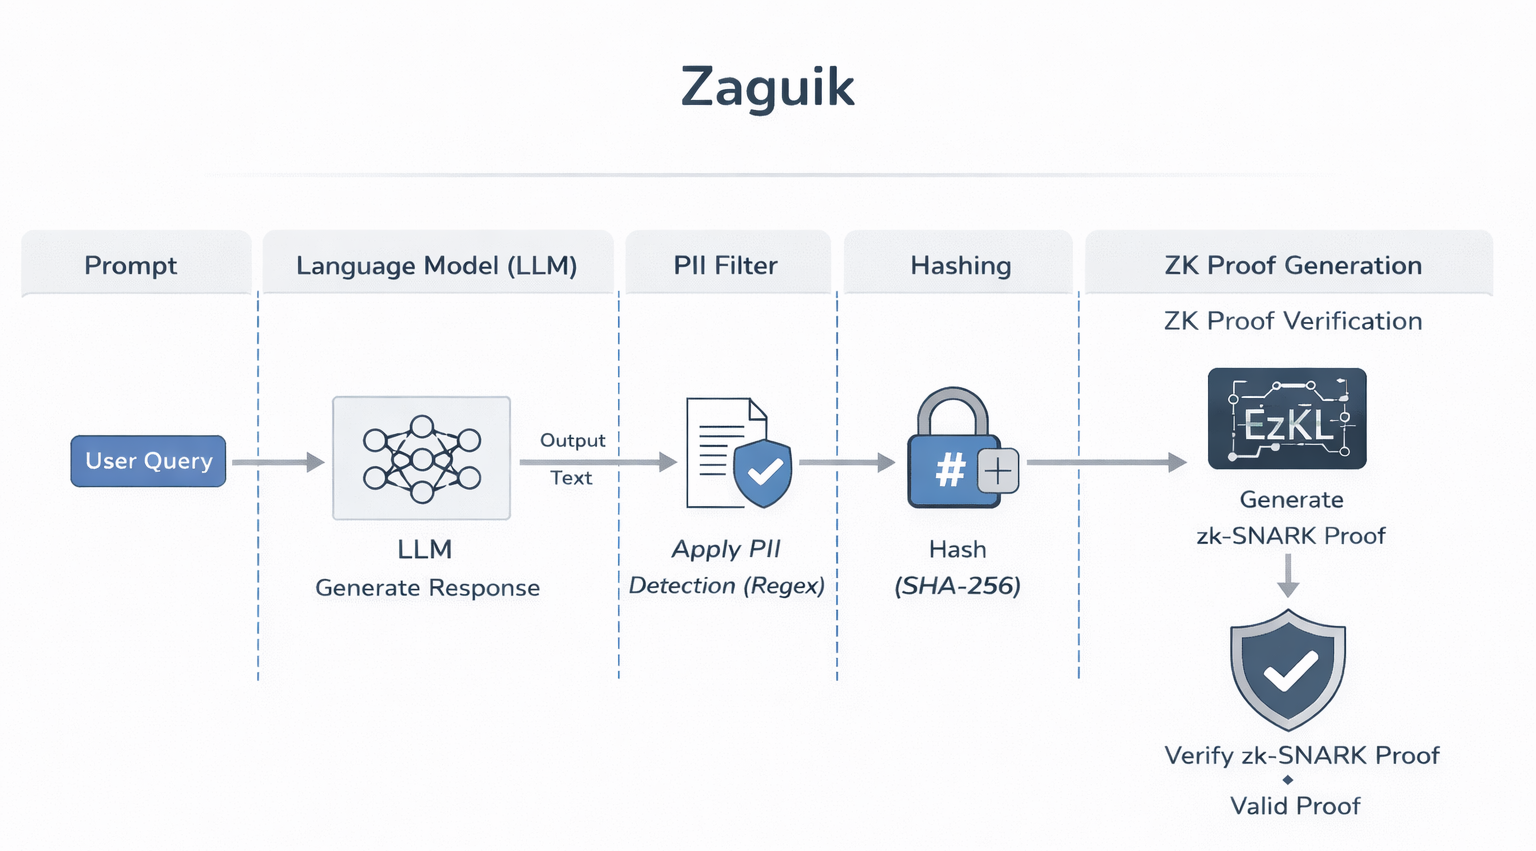
\includegraphics[width=\textwidth]{system_overview.png}
    \caption{Zaguik's end-to-end workflow: from user prompt and LLM response through PII filtering to proof generation and verification.}
    \label{fig:system_overview}
\end{figure}

A deliberate boundary of the design is that the LLM itself is outside the scope of the proof. We do not attest that the model behaved in any particular way; we attest only that a given string was passed through the certified PII filter and accepted. This keeps the attested computation small and well defined, which, as Section~\ref{sec:sd-circuit} explains, is essential given the cost of expressing computations as arithmetic circuits.

\section{PII Filtering: A Two-Layer Approach}
\label{sec:sd-filtering}

The filtering logic in Zaguik is split into two distinct components, serving two different purposes.

\medskip

\textbf{An operational detector.} In plain execution, the system applies a regex-based PII filter that searches for structured patterns such as email addresses, phone numbers, and identification numbers. Its role is operational: it acts as a gating mechanism that prevents obviously unsafe outputs from ever reaching the proof phase. This detector runs in the clear and is never itself the object of the proof.

\medskip

\textbf{A circuit-friendly policy.} For the zero-knowledge attestation, the system uses a separate, deliberately simple policy that can be efficiently expressed as an arithmetic circuit. It is implemented as a small module that operates at the byte level: it takes a fixed-length normalised byte vector as input and counts the occurrences of a fixed set of ``suspicious'' byte values that are characteristic of common PII. Concretely, the set comprises the \texttt{@} character (byte~64), associated with email addresses, together with the digits \texttt{0}--\texttt{9} (bytes~48--57), the hyphen (byte~45), and the period (byte~46), which are characteristic of phone numbers, identification numbers, and similar structured data. The module sums, over all positions, the number of input bytes equal to any of these values and outputs the resulting count; the policy is considered satisfied, \texttt{PASS}, if and only if this count is zero.

\medskip

It is important to be precise about what this separation implies. The zk-SNARK proof certifies correct execution of the byte-level circuit and the fact that its output is zero; it does \emph{not} certify execution of the regex detector. The correspondence between the two is a design choice, not a formally verified equivalence: the byte-level policy can be read as a conservative structural proxy for certain classes of PII indicators, but it does not capture the full semantics of the regex detector. Establishing a formal equivalence between a high-level filtering rule and its circuit representation is an open problem and outside the scope of this prototype. The attestation mechanism is also \emph{policy-agnostic}: any deterministic rule expressible as an ONNX model compatible with the proving backend can be certified in the same way. The byte-level policy is simply the instantiation that current tooling made feasible, for reasons we turn to next.

\section{Circuit Design: From a Neural Detector to a Byte-Level Policy}
\label{sec:sd-circuit}

The choice of byte-level policy was not the starting point of this work but its outcome. The initial design aimed to attest a realistic PII detector: a BERT-based named-entity-recognition model of the kind described in Chapter~\ref{chap:background}, exported to ONNX and compiled into a circuit with EzKL. This would have allowed the proof to attest the execution of a genuine, model-based detector rather than a structural proxy.

\medskip

In practice, this approach proved infeasible under the conditions available for this project. The obstacle was \emph{resource exhaustion}: the size of a Transformer-based detector caused the EzKL \texttt{compile} and \texttt{setup} stages to exhaust the available memory on the experimental machine (16~GB of RAM, CPU only; see Chapter~\ref{chap:evaluation}). The arithmetisation cost discussed in Section~\ref{subsec:bg-circuits} is precisely what manifested here: the number of constraints needed to represent a full neural detector exceeded what the toolchain could handle in this environment.

\medskip

After several unsuccessful attempts, the design was therefore reduced to the byte-level counter, which is small enough to compile and prove reliably while still demonstrating the end-to-end attestation mechanism. We regard this not as a defeat but as an informative result in its own right: it delineates the current practical boundary of ZKML tooling for this class of application, and it motivates several of the directions discussed in Chapter~\ref{chap:discussion}. The pipeline itself is unchanged by the choice of policy; substituting a more expressive circuit, once tooling and hardware permit, requires no change to the surrounding architecture.

\section{Encoding and Circuit Input}
\label{sec:sd-encoding}

The LLM output is a string, but the circuit operates on a fixed-size numeric tensor, so the output must be encoded. We fix an upper bound $L$ on the number of UTF-8 bytes; in our implementation $L = 2048$. When the generated output fits within $L$ bytes it is encoded and attested in full (zero-padded to $L$); when it is longer, only its first $L$ bytes (the prefix $y_L$) are encoded and attested. In the evaluation of Chapter~\ref{chap:evaluation} we deliberately generate outputs longer than $L$ in order to exercise this prefix-truncation path.

\medskip

The encoding proceeds as follows. The string is represented in UTF-8, zero-padded to length $L$ if shorter, and each byte is normalised to the interval $[0,1]$ by dividing by $255$. The resulting vector has shape $[1, L]$ and is used as the single input tensor to the ONNX circuit. We write $\mathrm{Enc}_L(\cdot)$ for this encoding.

\medskip

Separately from the circuit input, a SHA-256 hash of the prefix $y_L$ (its raw first-$L$ bytes, prior to encoding) is computed and published. This hash acts as a protocol-level commitment that associates the proof with the attested prefix; it is not fed into the circuit, and the equality between the published hash and the prefix is not verified within the proof. The precise role of this commitment, and its security implications, are made explicit in the next section.

\section{Formal Model and Security}
\label{sec:sd-formal}

We now state precisely what the proof guarantees, drawing on the zero-knowledge notions of Chapter~\ref{chap:background}. The relevant notation is as follows. Let $y \in \{0,1\}^{*}$ be the full output string generated by the LLM, let $L$ be the fixed encoding length in bytes, and let $y_L$ be the prefix of $y$ consisting of its first $L$ UTF-8 bytes (or all of $y$ if $|y| \le L$). Let $x = \mathrm{Enc}_L(y_L)$ be the encoded prefix, let $H(\cdot)$ be a cryptographic hash function (SHA-256), and let $C$ be the certified arithmetic circuit implementing the byte-level policy.

\medskip

\textbf{Public instance and private witness.} Following the structure of an NP relation from Chapter~\ref{chap:background}, the proof separates public from private data:
\begin{itemize}
    \item The \emph{public instance} consists of the circuit output $o$, a non-negative integer equal to the number of suspicious bytes counted, with \texttt{PASS} signalled by $o = 0$ and \texttt{FAIL} by $o > 0$.
    \item The \emph{private witness} consists of the encoded prefix $x$ and the internal intermediate values required to execute $C$.
\end{itemize}
The verification key and the structured reference string are public system parameters available to the verifier, but they are not part of the public instance of any specific proof. Table~\ref{tab:visibility} consolidates the visibility of every element in the protocol, summarising what remains private to the prover and what the verifier is able to see.

\begin{table}[htbp]
\centering
\caption{Visibility of each element in the Zaguik protocol. The verifier sees only the public column; the model output and its encoding never leave the prover.}
\label{tab:visibility}
\footnotesize
\begin{tabular}{l l p{6.2cm}}
\hline
\hline
Element & Visibility & Description \\
\hline
Output text $y$, prefix $y_L$ & Private & The generated text; known only to the prover, never revealed. \\
Encoded prefix $x = \mathrm{Enc}_L(y_L)$ & Private (witness) & The circuit's input tensor; part of the witness. \\
Internal circuit values & Private (witness) & Intermediate values needed to execute $C$. \\
Circuit output $o$ (suspicious-byte count) & Public (instance) & Revealed; $o = 0$ confirms \texttt{PASS}. \\
Hash commitment $h = H(y_L)$ & Public & Protocol-level; \emph{not} verified inside the circuit. \\
Proof $\pi$ & Public & Checked by the verifier. \\
Verification key, SRS & Public & System parameters available to all parties. \\
\hline
\hline
\end{tabular}
\end{table}

\medskip

\textbf{Circuit statement.} The zk-SNARK proves the NP statement
\[
    \exists\, x \;\text{ such that }\; C(x) = 0,
\]
that is, the prover demonstrates knowledge of an encoded input $x$ on which the certified circuit counts zero suspicious bytes and therefore evaluates to \texttt{PASS}. The circuit operates only on the encoded prefix $x$ and never receives the full string $y$.

\medskip

\textbf{Protocol-level commitment.} Separately from the circuit, the prover computes and publishes the commitment
\[
    h = H(y_L),
\]
which binds the attestation to the prefix $y_L$ at the protocol level. Note that the equality $H(y_L) = h$ is \emph{not} verified inside the circuit. The binding between the public hash $h$ and the private witness $x$ relies on the prover having computed both from the same $y_L$ before proof generation. The SNARK guarantees correct execution of $C(x)$; the hash operates as a separate commitment alongside it.

\medskip

\textbf{Security model.} We assume a standard adversarial model in which the prover may be malicious and the verifier is honest and follows the verification algorithm. Under the soundness of zk-SNARKs (Definition~\ref{def:completeness-soundness}), no probabilistic polynomial-time adversary can produce a valid proof for $C(x) = 0$ without knowledge of a witness $x$ satisfying that relation. Zero-knowledge (Definition~\ref{def:czk}) ensures that the proof reveals no information about $x$ beyond the truth of the statement. However, because the hash commitment is enforced only at the protocol level and not inside the circuit, the binding between $h$ and $x$ holds only under an \emph{honest-prover assumption}: a malicious prover could in principle generate a valid proof for some $x$ while publishing an unrelated $h$. Strengthening this binding would require verifying the hash inside the circuit, ideally with a SNARK-friendly hash function, at the cost of additional circuit complexity.

\medskip

\textbf{Scope of the guarantee.} The proof guarantees correct execution of the certified circuit $C$ on an encoded prefix $x$. If $|y| \le L$ the entire output is attested; otherwise only the first $L$ bytes are attested. The system does not prove the semantic adequacy of the filtering policy, nor does it make any claim about the internal behaviour of the LLM. The guarantee is limited to enforcement integrity of the circuit-level constraint over the attested prefix.

\section{Proof Generation Pipeline}
\label{sec:sd-pipeline}

The cryptographic pipeline follows the three stages of a zk-SNARK introduced in Chapter~\ref{chap:background}: setup, prove, and verify.

\medskip

\textbf{Setup.} Setup is performed once per circuit. The ONNX model is used to generate the proof-system settings and to compile the arithmetic circuit. A KZG structured reference string (SRS) is required; it can be obtained from a trusted source or, as in our prototype, generated locally for testing. With the compiled circuit and the SRS, key generation produces a proving key and a verification key.

\medskip

\textbf{Prove.} For each clean output to be attested, the system encodes it as circuit input, computes the witness, and runs the prover to produce the proof. The proof, the verification key, and (in deployment) the public commitment to the output are what the verifier subsequently needs.

\medskip

\textbf{Verify.} Verification is deterministic: given the proof, the verification key, the settings, and the SRS, the verifier runs the verification algorithm and accepts if and only if the proof is valid. No secret data is required. The verifier does not learn the output and cannot confirm its exact contents; at most, if it holds the published SHA-256 hash, it can associate the proof with the attested prefix under the honest-prover assumption discussed above, a correspondence that is not enforced inside the circuit.

\medskip

The \emph{visibility semantics} of the protocol follow the split summarised earlier in Table~\ref{tab:visibility}: the encoded input is kept private as witness data, the circuit output is exposed so that the verifier can confirm a \texttt{PASS}, and the filter parameters are fixed in the circuit rather than revealed, so the verifier learns only that the same certified circuit was executed. Together these choices ensure that the proof establishes execution of the certified circuit on a private encoded prefix returning \texttt{PASS}, while only a hash commitment to that prefix is exposed.

\section{Implementation Details}
\label{sec:sd-implementation}

The reference implementation is written in Python and structured as a single scriptable workflow covering ONNX export, encoding, setup, proof generation, and verification. The default configuration builds the small byte-level ONNX model, runs setup, and then generates and verifies proofs for a given text string.

\medskip

The cryptographic backend is EzKL, pinned to version~22.2.1; this pin is deliberate, as other versions exhibited incompatibilities in our environment. The structured reference string is generated locally using EzKL's facilities rather than retrieved from a public ceremony. This is appropriate for a self-contained research prototype but would differ in a production deployment, where the SRS would be obtained from a trusted ceremony, as discussed in Chapter~\ref{chap:discussion}. All stages are documented so that the pipeline can be reproduced and extended; integrating a more expressive PII model would require only an ONNX export compatible with the proving backend, with no change to the surrounding pipeline.

\chapter{Evaluation}
\label{chap:evaluation}

This chapter reports the empirical evaluation of the Zaguik pipeline. We first describe the experimental setup (Section~\ref{sec:eval-setup}), then present the one-time setup costs (Section~\ref{sec:eval-setup-costs}) and the proof size and timing results across encoding lengths (Section~\ref{sec:eval-results}). The interpretation of these results is deferred to Chapter~\ref{chap:discussion}.

\section{Experimental Setup}
\label{sec:eval-setup}

All experiments were conducted locally on a single machine with a Snapdragon~X 12-core X1E80100 CPU at 3.40\,GHz, 16\,GB of RAM, running Windows~11 (64-bit). The implementation uses Python~3.13.3 and EzKL~22.2.1. No GPU acceleration was used; all proof generation and verification ran entirely on CPU.

\medskip

The structured reference string (SRS) was generated locally using EzKL's facilities rather than retrieved from a remote trusted source. As discussed in Chapters~\ref{chap:system-design} and~\ref{chap:discussion}, this is appropriate for a self-contained research prototype but would differ in a production deployment, where the SRS would be obtained from a public trusted ceremony.

\medskip

Experiments were run sequentially, with no parallel execution across configurations. A single reference output was generated once from a fixed prompt with DistilGPT-2 and reused throughout; it was designed to exceed 2048 bytes so that, for every value of $L$, the encoding window was fully populated (when $L < 2048$, only the first $L$ bytes were encoded and attested). We evaluated five encoding lengths, $L \in \{128, 256, 512, 1024, 2048\}$ bytes, and for each $L$ we repeated proof generation and verification fifteen times ($n = 15$) on this same input, so that the repetitions isolate run-to-run timing variability rather than variation in the data. This yields $5 \times 15 = 75$ proof-generation and verification attempts in total, and the mean values and sample statistics over the fifteen repetitions are reported below.

\medskip

Two clarifications are needed to read these results correctly. First, the pipeline is \emph{gated}: as described in Chapter~\ref{chap:system-design}, the operational regex detector runs in the clear first, and only outputs it judges free of structured PII (emails, phone numbers, identification numbers, and similar) ever reach the proof phase. The attested inputs are therefore ``clean'' in the sense of that detector. Second, and crucially, the circuit policy is stricter and different in kind: it counts the suspicious bytes \texttt{@}, \texttt{-}, \texttt{.}, and the digits \texttt{0}--\texttt{9}, and signals \texttt{PASS} only when this count is zero. Because the period and digits occur in virtually all natural-language text, a multi-hundred-byte LLM output yields a positive count even after passing the regex gate, so the attested result in these runs is a nonzero suspicious-byte count rather than a \texttt{PASS}. This distinction does not affect the quantities measured in this chapter (proof size, proving time, witness time, and verification time are determined by the circuit and the encoding length $L$, not by the value of the count), but it means the experiments should be read as a characterisation of \emph{attestation cost}, not as a measurement of how often outputs satisfy the policy. Accordingly, when we report that all 75 attempts ``succeeded'', we mean precisely that every proof was generated and then verified without error, not that any output produced a \texttt{PASS}.

\section{One-Time Setup Costs}
\label{sec:eval-setup-costs}

Table~\ref{tab:setup-costs} reports the one-time setup costs for the circuit with $L = 2048$, comprising settings generation, circuit compilation, SRS generation, witness setup, and key generation. The total setup time was 102.44\,seconds. This cost is dominated by SRS generation (77.88\,s) and key generation (23.77\,s); the remaining steps each took under one second. Because setup is performed once per circuit and then amortised over all subsequent proofs, it does not contribute to the per-proof cost reported in the next section.

\begin{table}[htbp]
\centering
\caption{One-time setup costs (byte-level PII circuit, $L = 2048$).}
\label{tab:setup-costs}
\vspace{2ex}
\begin{tabular}{l r}
\hline
\hline
Step & Time (s) \\
\hline
Settings generation & 0.14 \\
Circuit compilation & 0.02 \\
SRS generation$^{a}$ & 77.88 \\
Witness (setup) & 0.63 \\
Key generation & 23.77 \\
\hline
Total & 102.44 \\
\hline
\hline
\multicolumn{2}{l}{\footnotesize $^{a}$Generated locally for testing; production deployments would} \\
\multicolumn{2}{l}{\footnotesize obtain the SRS from a trusted ceremony.} \\
\end{tabular}
\end{table}

\section{Proof Size and Timing Results}
\label{sec:eval-results}

Table~\ref{tab:results} presents the proof size, proof generation time, witness computation time, and verification time for each value of $L$, reported as mean $\pm$ sample standard deviation over the fifteen repetitions. All 75 proof-generation and verification attempts completed without error across the five encoding lengths, in the sense clarified in Section~\ref{sec:eval-setup}: every proof was generated and then verified successfully.

\medskip

\begin{table}[htbp]
\centering
\caption{Proof size and timings vs.\ circuit encoding size $L$ (15 independent runs; $n=15$; reference output $\ge 2048$ bytes, prefix-truncated to the $L$-byte window). Each $L$ block shows mean, sample standard deviation ($\pm$Std), and observed range [Min, Max].}
\label{tab:results}
\footnotesize
\setlength{\tabcolsep}{4pt}
\vspace{2ex}
\begin{tabular}{c l r r r r}
\hline
\hline
$L$ (bytes) & & Proof size (bytes) & Proof gen.\ (ms) & Witness (ms) & Verify (ms) \\
\hline
\multirow{3}{*}{128}
  & Mean      & 21896.67 & 15240.07 &  54.31 & 195.64 \\
  & $\pm$Std  & $\pm$27.33 & $\pm$8049.70 & $\pm$21.53 & $\pm$50.65 \\
  & {[Min, Max]} & {[21850, 21944]} & {[10014.94, 33601.85]} & {[40.91, 128.50]} & {[150.74, 305.65]} \\
\hline
\multirow{3}{*}{256}
  & Mean      & 21870.73 & 19240.44 &  89.36 & 200.85 \\
  & $\pm$Std  & $\pm$39.03 & $\pm$9922.94 & $\pm$18.08 & $\pm$65.80 \\
  & {[Min, Max]} & {[21822, 21966]} & {[11019.33, 32606.75]} & {[70.93, 134.03]} & {[149.94, 398.31]} \\
\hline
\multirow{3}{*}{512}
  & Mean      & 21892.67 & 15944.43 & 150.55 & 168.73 \\
  & $\pm$Std  & $\pm$33.82 & $\pm$7903.57 & $\pm$16.24 & $\pm$22.70 \\
  & {[Min, Max]} & {[21835, 21954]} & {[10983.38, 33031.74]} & {[122.49, 183.49]} & {[140.98, 232.17]} \\
\hline
\multirow{3}{*}{1024}
  & Mean      & 21893.07 & 14840.25 & 268.43 & 174.02 \\
  & $\pm$Std  & $\pm$32.81 & $\pm$6573.20 & $\pm$20.57 & $\pm$34.71 \\
  & {[Min, Max]} & {[21841, 21955]} & {[12137.78, 37693.64]} & {[237.38, 295.59]} & {[138.79, 260.96]} \\
\hline
\multirow{3}{*}{2048}
  & Mean      & 21929.27 & 18219.90 & 540.82 & 182.45 \\
  & $\pm$Std  & $\pm$37.22 & $\pm$9359.92 & $\pm$69.33 & $\pm$30.32 \\
  & {[Min, Max]} & {[21867, 21991]} & {[12659.16, 43176.02]} & {[447.87, 704.70]} & {[152.73, 259.90]} \\
\hline
\hline
\end{tabular}
\end{table}

We highlight four factual observations from Table~\ref{tab:results}; their interpretation is taken up in Chapter~\ref{chap:discussion}.

\medskip

\textbf{Proof size is essentially constant.} The mean proof size varies between 21\,871 bytes ($L = 256$) and 21\,929 bytes ($L = 2048$), a spread of less than 0.3\,\% across a sixteen-fold increase in $L$, with no monotonic trend.

\medskip

\textbf{Proof generation dominates and is highly variable.} Mean proof-generation time ranges from roughly 14\,840\,ms ($L = 1024$) to 19\,240\,ms ($L = 256$), with large standard deviations ($\pm$6\,573 to $\pm$9\,923\,ms). It does not vary monotonically with $L$.

\medskip

\textbf{Witness computation grows monotonically with $L$.} Mean witness time increases steadily from 54.31\,ms at $L = 128$ to 540.82\,ms at $L = 2048$, tracking the size of the encoding window.

\medskip

\textbf{Verification time is stable.} Mean verification time stays within a narrow band (roughly 169--201\,ms) across all configurations, with occasional spikes in individual runs but no systematic dependence on $L$.

\chapter{Discussion}
\label{chap:discussion}

This chapter interprets the results of Chapter~\ref{chap:evaluation} (Section~\ref{sec:disc-interpretation}), examines the governance and security implications of the system (Section~\ref{sec:disc-governance}), states its limitations (Section~\ref{sec:disc-limitations}), and sketches a path towards production deployment (Section~\ref{sec:disc-production}).

\section{Interpretation of Results}
\label{sec:disc-interpretation}

The experiments show that zero-knowledge attestation of an output-filtering policy can be carried out end to end using a compact circuit, and the measured costs follow a consistent pattern.

\medskip

The near-constant proof size, varying by under 0.3\,\% across a sixteen-fold change in $L$, confirms that proof size is determined by the structure of the circuit rather than by the amount of attested data. The small fluctuations observed are attributable to internal serialisation and metadata encoding in the proof object, not to changes in the underlying constraint system. This is the expected behaviour of a succinct argument, and it is precisely the property that makes such proofs attractive for an attestation that may be stored and checked many times. The absolute size of roughly 21.9\,KB reflects the Halo2/KZG proving system underlying EzKL, which yields larger proofs than the few-hundred-byte Groth16 proofs noted in Chapter~\ref{chap:background}; succinctness here refers to the proof's independence from the input size, not to a specific byte count.

\medskip

Witness computation time, by contrast, grows monotonically with $L$, from 54\,ms to 541\,ms as $L$ increases from 128 to 2048 bytes. This is the one cost that tracks the size of the encoding window directly, since the number of input values committed to the circuit grows with $L$. Even at $L = 2048$, however, witness computation remains well under a second and is a minor contributor to the total.

\medskip

The dominant cost is proof generation, which is also the most variable: mean times lie between roughly 15 and 19\,seconds, but with standard deviations of 6.6--9.9\,seconds and no monotonic dependence on $L$. The absence of a clean relationship with $L$, combined with the large variance, indicates that proof-generation time at this scale is governed by local execution conditions, operating-system scheduling and memory pressure on a loaded CPU, rather than by the size of the encoding window. In other words, the circuit is small enough that data size is not the bottleneck; the runtime environment is.

\medskip

Verification time remains broadly stable across all configurations (169--201\,ms on average), consistent with the constant-size verifier computation characteristic of KZG-based SNARKs. The contrast with proof-generation cost reveals a pronounced asymmetry: the computational burden falls almost entirely on the prover, while verification stays lightweight regardless of $L$. This asymmetry is favourable for the intended use case, in which a single prover produces an attestation that many verifiers, such as auditors, may later check cheaply.

\medskip

Finally, the experiments validate the prefix-attestation mechanism itself. For $L < 2048$, only the first $L$ bytes are encoded and attested, and all 75 attempts across the five values of $L$ succeeded. This confirms that the attested length can be tuned to circuit-cost constraints while preserving verifiability, at the cost of limiting the guarantee to the attested prefix rather than the entire output.

\section{Governance and Security Implications}
\label{sec:disc-governance}

The pipeline illustrates a shift from trust-based enforcement to cryptographically verifiable enforcement. In conventional deployments, an external party must rely on the provider's assertion that a privacy filter is applied to LLM outputs; the alternative, inspecting the outputs or the filtering logic directly, reintroduces the very privacy and intellectual-property concerns the filter was meant to address. Zaguik enables a third party to verify instead that a specific, predefined circuit-based policy was executed on a private encoded prefix and returned \texttt{PASS}, without revealing the output itself.

\medskip

It is important to state precisely what this does and does not establish. The proof attests correct execution of the certified circuit on an encoded prefix and the satisfaction of the encoded constraint. It does not allow the verifier to recover or confirm the exact output: as set out in Chapter~\ref{chap:system-design}, the verifier sees only the public elements of Table~\ref{tab:visibility}, and the hash commitment links the proof to the attested prefix at the protocol level only, under an honest-prover assumption, rather than being verified inside the circuit. The mechanism therefore supports a form of privacy-preserving auditability: verification can occur without access to the generated text.

\medskip

We deliberately frame this contribution in measured terms. Zaguik does not, by itself, ensure regulatory compliance, and it is not a compliance product; it provides a cryptographic primitive that could be integrated into governance frameworks where evidence of enforcement is required. As noted in Chapter~\ref{chap:related-work}, this aligns with the evidentiary thrust common to data-protection and AI-specific regulation, without satisfying any particular legal obligation on its own. The architecture is also policy-agnostic at the circuit level: any deterministic filtering rule expressible as a compatible ONNX model can in principle be attested by the same mechanism, so the governance argument does not depend on the specific byte-level policy used in our prototype.

\section{Limitations}
\label{sec:disc-limitations}

Several limitations must be acknowledged, most of which follow directly from the design choices and results discussed above.

\medskip

\textbf{Lightweight policy.} The attested circuit is intentionally simple. As explained in Chapter~\ref{chap:system-design}, the byte-level counter was adopted after a neural NER detector proved infeasible to compile and prove under the available resources. While sufficient to demonstrate feasibility, it does not reflect the sophistication of modern PII detection.

\medskip

\textbf{Prefix-bounded guarantee.} The circuit operates on a fixed-length byte vector, so when $L$ is smaller than the full output length only the first $L$ bytes are attested. Extending coverage to arbitrarily long outputs would require increasing $L$, segmenting outputs into multiple proofs, or employing recursive proof composition.

\medskip

\textbf{No formal filter--circuit equivalence.} The system proves correct execution of the byte-level circuit, not of the regex detector used operationally. The two are separate components, and while the circuit captures structural indicators of PII, no formal equivalence between the deployment-time filtering logic and its circuit representation is established.

\medskip

\textbf{Protocol-level hash binding.} Consistency between the public hash commitment and the encoded circuit input is enforced at the protocol level, not inside the circuit. The proof certifies correct execution of the circuit on a private input, but does not cryptographically guarantee that the published hash corresponds to the exact bytes used within the proof. Strengthening this binding by verifying the hash inside the circuit would increase circuit complexity and proof cost.

\medskip

\textbf{Policy semantics, not adequacy.} The system guarantees enforcement integrity of the encoded policy, not the semantic adequacy of that policy. A weak or incomplete detector can be correctly executed and faithfully proven; the attestation certifies that a rule was applied, not that the rule captures all relevant forms of personal data.

\medskip

\textbf{Static circuit.} Production filtering policies evolve to address new patterns and requirements, but the arithmetic circuit is static. Any change to the policy requires recompiling the circuit, regenerating the proving and verification keys, and repeating the setup phase, an operational overhead that may limit applicability where filtering logic changes frequently.

\section{Towards Production Deployment}
\label{sec:disc-production}

Deploying Zaguik in a real environment would require addressing several requirements beyond the current prototype, which together outline a realistic path forward.

\medskip

\textbf{A more expressive policy.} The byte-level counter would need to be replaced with a policy that more faithfully reflects real PII detection, such as a lightweight neural detector or a richer regex-derived circuit, subject to the ONNX-compatibility and resource constraints identified in Chapter~\ref{chap:system-design}.

\medskip

\textbf{A trusted-ceremony SRS.} The structured reference string would need to be obtained from a public trusted ceremony rather than generated locally, since local generation does not provide the soundness guarantees required in an adversarial setting.

\medskip

\textbf{Faster proving.} The current 15--19\,seconds per proof on CPU is impractical for high-throughput settings. GPU acceleration, which can reduce proving time by one to two orders of magnitude, together with optimised native implementations, would bring this into a practical range.

\medskip

\textbf{Asynchronous proof generation.} Proof generation should be decoupled from the real-time request path: proofs would be produced in the background after each response is delivered, stored with their hash commitments, and made available for audit on demand, eliminating user-facing latency while preserving the audit trail.

\medskip

\textbf{An accessible verifier interface.} Finally, a simple verifier tool that accepts a proof and returns a valid/invalid verdict would make the system usable by auditors and regulators without cryptographic expertise. Taken together, these components define a realistic route from the present prototype to a deployable compliance primitive, particularly suited to organisations operating their own private LLM infrastructure.

\chapter{Conclusions}
\label{chap:conclusions}

This thesis presented Zaguik, a privacy-preserving attestation system that proves, in zero knowledge, that an encoded LLM output prefix satisfies a certified filtering policy and returns a \texttt{PASS} result, without revealing the output itself. Building on the zero-knowledge foundations developed in Chapter~\ref{chap:background} and positioned against existing work in Chapter~\ref{chap:related-work}, the system chains LLM generation, PII filtering, zk-SNARK proof generation through EzKL, and verification into a single end-to-end pipeline (Chapter~\ref{chap:system-design}), which we then evaluated empirically across a range of encoding lengths (Chapter~\ref{chap:evaluation}) and interpreted in Chapter~\ref{chap:discussion}.

\medskip

We state the central claim precisely. The proof attests correct execution of a fixed, certified circuit on a private encoded prefix; it does not prove correct execution of the language model, it does not establish a formal equivalence between the deployment-time regex detector and the byte-level circuit, and the hash that links the proof to a specific output operates at the protocol level under an honest-prover assumption rather than being verified inside the circuit. Within these bounds, the system demonstrates something that, to our knowledge, had not previously been shown in a runnable form: that enforcement of a circuit-encoded policy over a language-model output can be attested cryptographically while keeping the output confidential.

\medskip

The empirical results support the practical feasibility of this approach at a small scale. Proof size remained essentially constant and verification time broadly stable across all tested encoding lengths, confirming the succinctness expected of a zk-SNARK, while witness computation grew with the encoding window and proof generation, the dominant cost, was governed more by the runtime environment than by the size of the attested data. The prover-heavy asymmetry of these costs is well suited to an audit setting, where a single attestation is produced once and may be verified cheaply and repeatedly. At the same time, the work surfaced a concrete boundary of current ZKML tooling: a full neural detector could not be compiled and proven under the available resources, which is why the attested policy was reduced to a lightweight byte-level counter. We regard this boundary as a useful empirical finding in its own right.

\medskip

Taken together, these results suggest that zero-knowledge proofs can serve as a building block for verifiable enforcement mechanisms in AI systems, providing a cryptographic primitive for accountability where evidence of enforcement is required but the underlying data must remain confidential. We are careful not to overstate this: Zaguik is a research prototype and a primitive, not a compliance solution, and the path from one to the other passes through the limitations set out in Chapter~\ref{chap:discussion}.

\section{Future Work}
\label{sec:concl-future}

Several directions follow naturally from this work.

\medskip

\textbf{More expressive policies in zero knowledge.} The most immediate goal is to attest a realistic detector rather than a byte-level proxy. This depends on advances in ZKML tooling and on hardware able to absorb the arithmetisation cost that defeated the neural detector here, and it would also narrow the gap between the operational filter and the attested circuit.

\medskip

\textbf{Stronger commitment binding.} The most important limitation to address is the honest-prover assumption on the commitment identified in Chapter~\ref{chap:system-design}. The binding between the public hash and the circuit input could be moved inside the circuit, for instance by verifying a SNARK-friendly hash of the encoded input as part of the proven statement. This would remove the honest-prover assumption and bring the system closer to the fully untrusted-prover setting that motivates it, at the cost of additional circuit complexity and proof cost.

\medskip

\textbf{Scaling to longer outputs.} The prefix-bounded guarantee could be extended to full outputs of arbitrary length through chunking into multiple proofs or through recursive proof composition, allowing coverage to grow without a proportional increase in per-proof cost.

\medskip

\textbf{Integration into governance and agentic workflows.} Finally, the attestation mechanism could be embedded within broader AI governance and compliance infrastructures, and extended to agentic workflows in which intermediate model outputs trigger external actions. In such settings, a policy check could be cryptographically enforced and attested before an action is executed, turning the primitive developed here into part of a larger accountable pipeline.



\bibliography{references}

\clearpage
\appendix

\chapter{The JNIC 2026 Conference Experience}
\label{app:jnic}

An earlier version of this work was submitted to the \emph{Jornadas Nacionales de Investigaci\'on en Ciberseguridad} (JNIC) 2026 and accepted for presentation at the conference, held from 6 to 8 May 2026. Presenting Zaguik there was, for me, one of the most rewarding moments of this project: it was the first time the ideas developed in this thesis were exposed to, and discussed with, a wider research community in cybersecurity. The questions, feedback, and conversations during those three days directly shaped how I framed several parts of this document, and the experience reinforced my conviction that the intersection of zero-knowledge proofs and AI governance is a direction worth pursuing.

\begin{figure}[htbp]
    \centering
    \includegraphics[width=0.9\textwidth]{DSC_1604.jpg}
    \caption{Presenting Zaguik at the JNIC 2026 conference.}
    \label{fig:jnic-1}
\end{figure}

\begin{figure}[htbp]
    \centering
    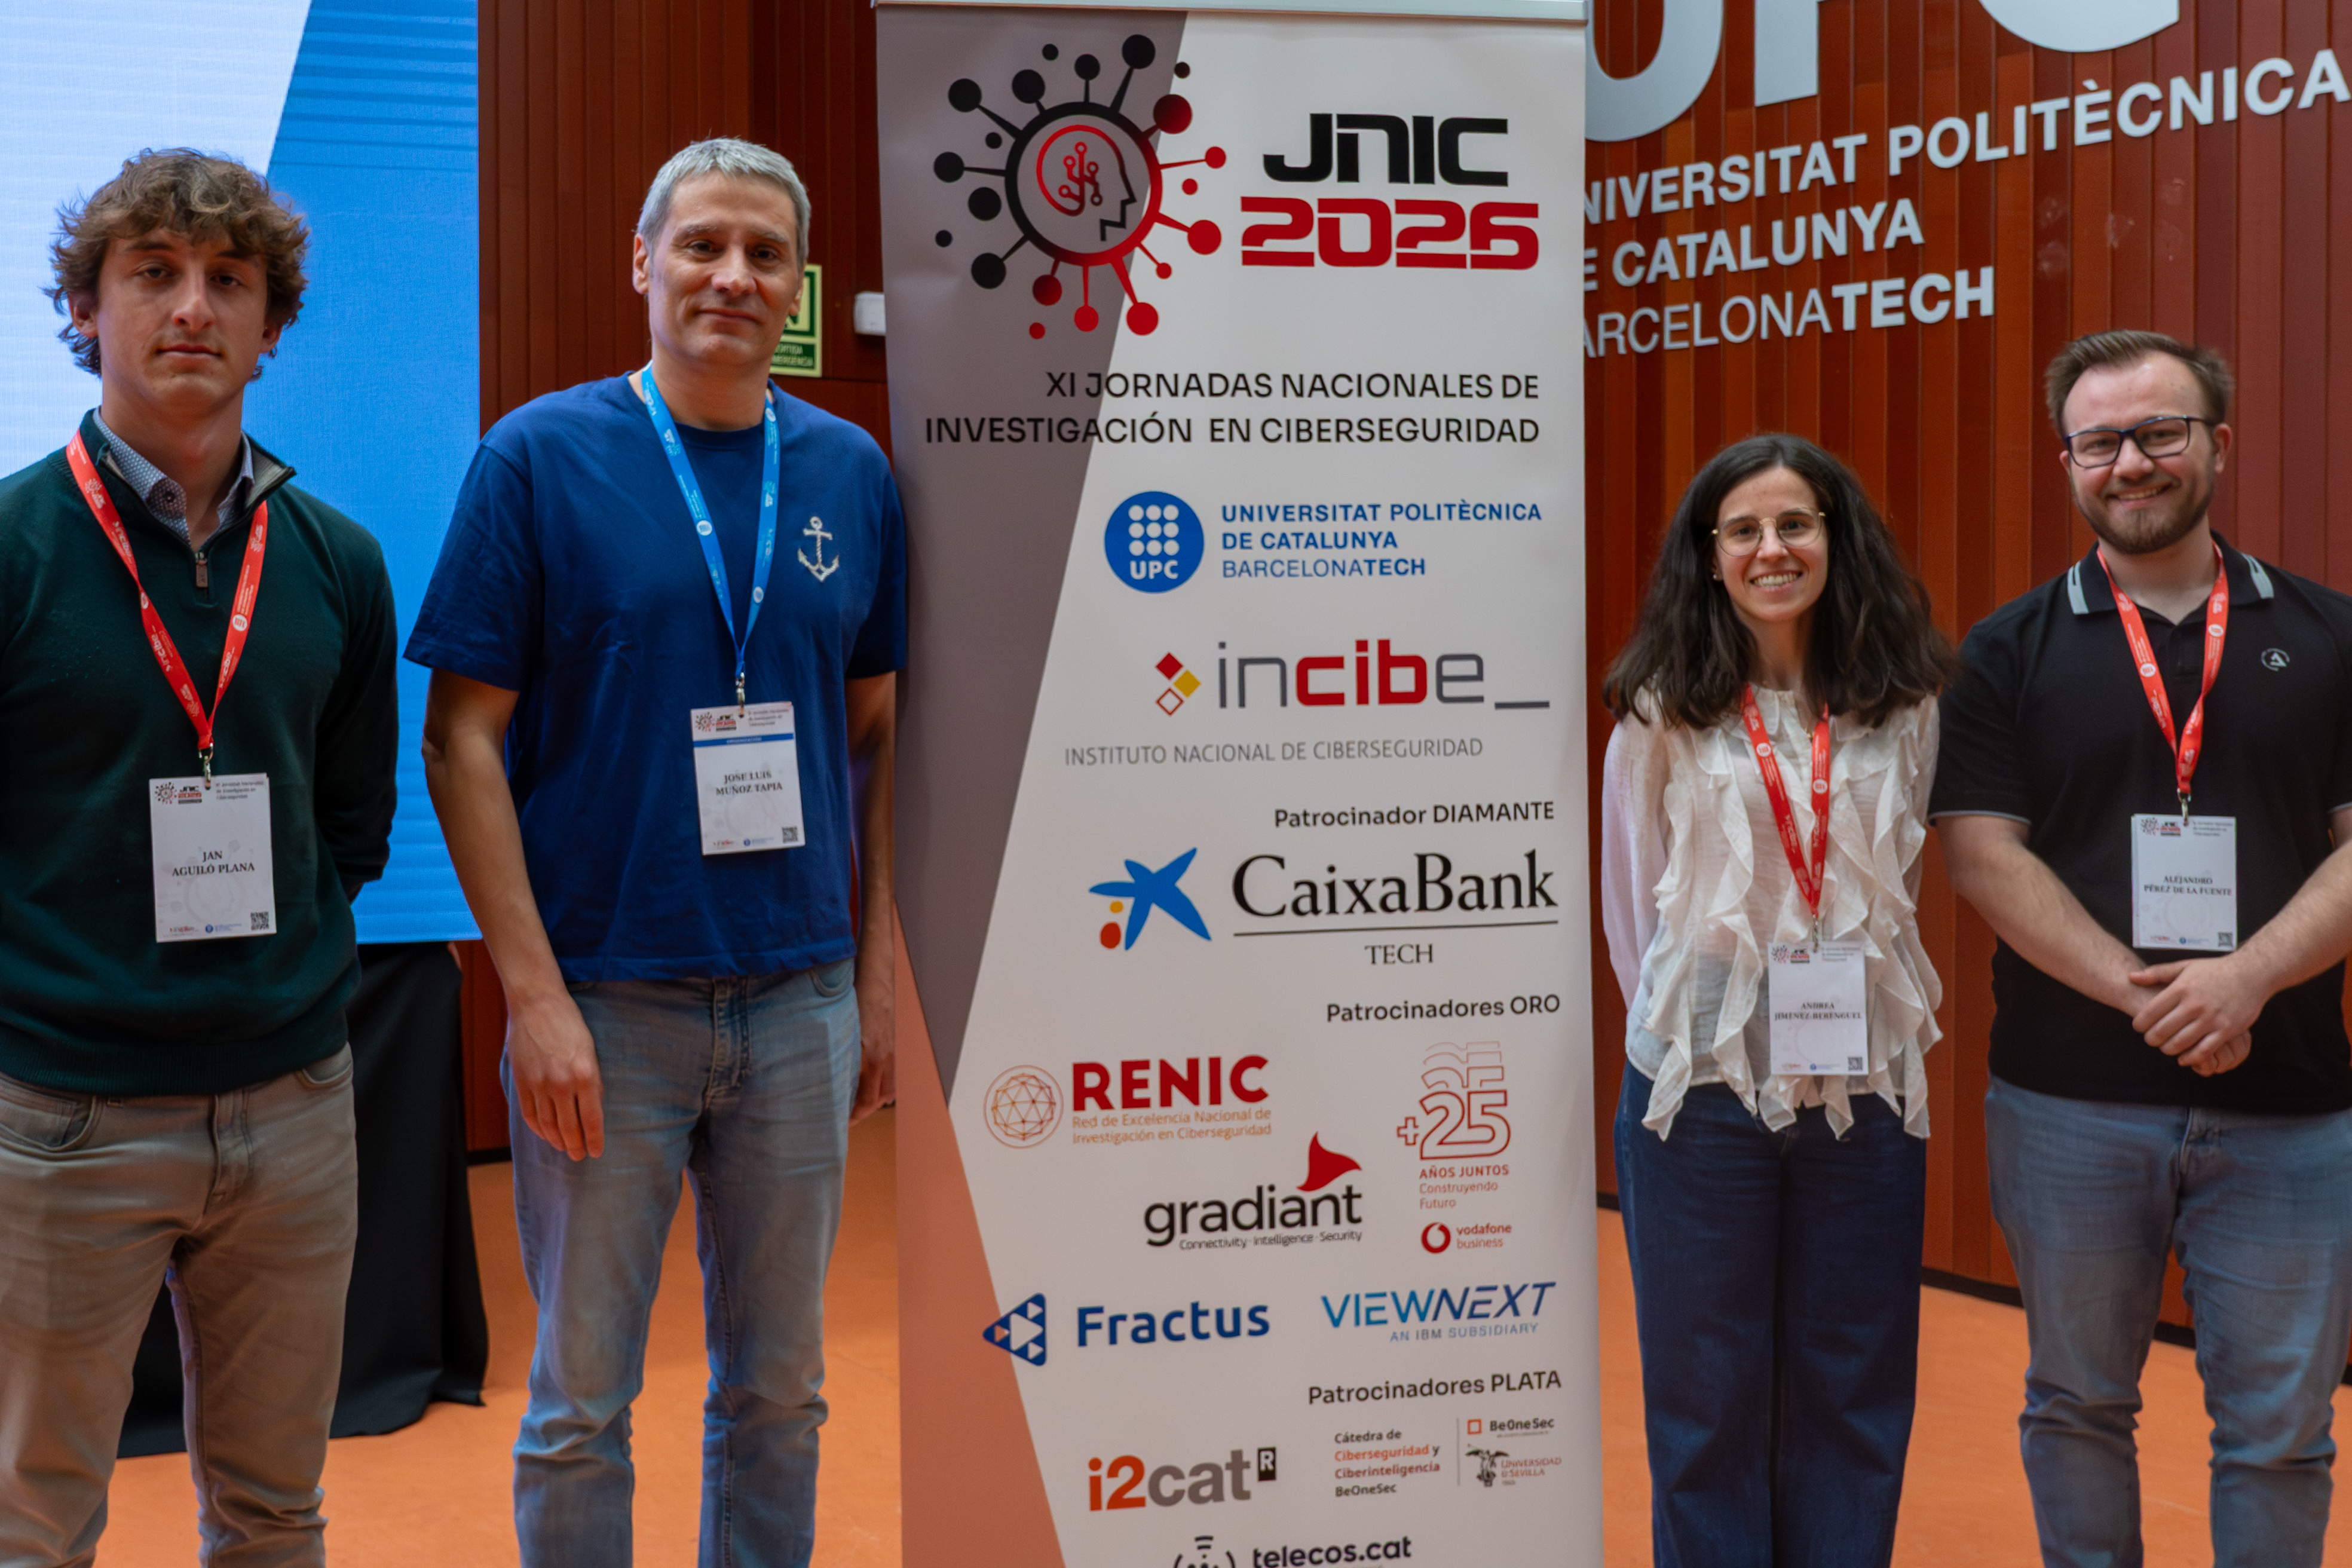
\includegraphics[width=0.9\textwidth]{DSC_1634.jpg}
    \caption{Picture after presenting Zaguik at the JNIC 2026 conference.}
    \label{fig:jnic-2}
\end{figure}


\end{document}
